\documentclass[a5paper]{article}
\usepackage[a5paper, top=17mm, bottom=17mm, left=17mm, right=17mm]{geometry}
\usepackage[utf8]{inputenc}
\usepackage[T2A,T1]{fontenc}
\usepackage[colorlinks,filecolor=blue,citecolor=green,unicode,pdftex]{hyperref}
\usepackage{cmap}
\usepackage[english,russian]{babel}
\usepackage{amsmath}
\usepackage{amssymb,amsfonts,textcomp}
\usepackage{color}
\usepackage{array}
\usepackage{hhline}
\hypersetup{colorlinks=true, linkcolor=blue, citecolor=blue, filecolor=blue, urlcolor=blue, pdftitle=1, pdfauthor=, pdfsubject=, pdfkeywords=}
% \usepackage[pdftex]{graphicx}
\usepackage{graphicx}
\usepackage{epigraph}
% Раскомментировать тем, у кого этот пакет есть. Шрифт станет заметно красивее.
%\usepackage{literat}
\usepackage{indentfirst}

\sloppy
\pagestyle{plain}
%\pagestyle{empty}

\title{Мышиные жесты, ПЫЩЬ}

\author{М.С. Осечкина \and Ю.В. Литвинов}
\date{}
\begin{document}

\maketitle
\thispagestyle{empty}

\epigraph{Цивилизация движется вперед путем увеличения числа операций, которые мы можем осуществлять, не раздумывая над ними}%
         {Альфред Норт Уайтхед}

\begin{quote}
\small\noindent
Аннотация, чо
\end{quote}

\section*{Введение}
Одной из особенностей разработки, управляемой моделями (model-driven development, MDD), является активное использование 
визуальных языков. Практически все действия, выполняемые в CASE-средствах или других используемых инструментах так или 
иначе сводятся к манипуляциям над элементами этих языков и связями между ними. 

Эффективность любого используемого инструмента определяется тем, насколько удобно и быстро он позволяет выполнять те операции, 
для которых этот инструмент предназначен. В процессе разработки моделей одними из наиболее часто выполняемых действий над объектами 
на диаграммах являются их создание и удаление.  В большинстве CASE-средств для того, чтобы создать нужный объект на диаграмме, 
необходимо найти его либо на панели инструментов, либо выбрать в меню, а затем указать место на диаграмме, где бы мы хотели этот 
элемент разместить. В большинстве инструментариев также возможен вариант создания объектов «перетаскиванием» (drag and drop) их из 
палитры элементов соответствующей диаграммы. То есть даже для такой базовой операции, как создание нового элемента, разработчику нужно 
совершить не только набор чисто механических действий, но еще и, скажем, вспомнить, на какой вкладке палитры или в каком меню находится 
нужный ему элемент, тем самым переключая контекст с продумывания иерархии создаваемых моделей на особенности манипуляции 
используемым инструментом. Нам кажется, что данную операцию можно и нужно автоматизировать, причем сделать это нужно максимально удобным для 
пользователей CASE-средств. В данной статье в качестве такого решения рассматривается подход, основанный на жестах мышью. 
Предлагается с каждым элементом ассоциировать определенный жест мышью, выполненный с каким-либо модификатором (скажем, с зажатой 
правой кнопкой мыши или клавишей Alt) и при выполнении этого жеста создавать в данном месте соответствующий объект. 


\section{Использование жестов мышью в других приложениях}

В последнее время разработкам нетрадиционных подходов к организации человеко-машинного взаимодействия уделяется довольно много 
внимания, и идея подавать команды программам с помощью жестов мыши уже нашла свое применение во многих приложениях. Так, например, 
в веб-браузер Opera\footnote{http://www.opera.com/} встроена поддержка простейших жестов, вызывающих наиболее часто применяемые команды. К примеру, чтобы вернуться 
к предыдущей странице, можно нажать кнопку ``Back`` в панели браузера, а можно выполнить движение мышью влево при зажатой правой кнопке. 
Чтобы перейти к следующей странице (кнопка ``Forward``), нужно двигать мышь вправо, для обновления страницы (кнопка ``Reload'') -- вверх-вниз,
чтобы открыть новую вкладку -- вниз. Ясно, что при таких абстрактных жестах от алгоритма распознавания не требуется
большая точность -- достаточно просто разбить жест на направления и выделить 1-3 вектора наибольшей длины.

В некоторых компьютерных играх жесты позволяют указывать персонажам куда двигаться или заставляют их выполнять какие-то определенные
действия. Так как в QReal редакторы генерируются, необходимо, чтобы и жесты не приходилось писать вручную. В играх такие тонкости, очевидно,
излишни -- набор жестов там статичен.

Также существуют специальные утилиты, с помощью которых можно ввести поддержку мышиных жестов в любую программу 
(например, ~\cite{strokeIt, gMote, xstroke, flyGesture}).
Их недостаток с точки зрения рассматриваемой задачи состоит в том, что добавляется лишь ограниченное число заранее определенных команд: 
сохранение, распечатка, копирование, вставка и некоторые другие. В QReal необходимо реализовать на порядок больше различных жестов. И если в
вышеперечисленных утилитах можно обойтись перебором всевозможных путей мыши, по которым вызывается та или иная команда, то в CASE-средстве 
перебирать придется слишком много вариантов. Ограничиться простейшими жестами (вверх, вниз, вправо, влево) невозможно, так как 
объектов слишком много и может возникнуть конфликт между двумя командами, у которых будет один и тот же жест. Некоторые программы 
в таких случаях по жесту предоставляют список команд, из которых пользователь может выбрать. Но если список будет слишком большим или 
будет вызываться при каждом жесте мышью, то смысл введения жестов пропадает, так как большинство инструментов, включая QReal, уже 
предоставляет пользователю список объектов, которые с помощью операции drag-and-drop можно перетаскивать на рабочее поле.

Отдельно хотелось бы выделить CASE-систему Visual Paradigm\footnote{http://www.visual-paradigm.com/product/vpuml/}, в которой частично реализован 
предлагаемый в данной статье подход. 
В Visual Paradigm мышиные жесты подразделяются на 3 типа – жесты, порождающие объект, жесты, вызывающие команду или жесты, 
создающие связь между объектами. Жесты, порождающие объект и вызывающие команды, задаются набором направлений (вверх, вниз, вправо, влево). 
Мышиных жестов в Visual Paradigm гораздо больше, чем в вышеописанных утилитах. Но, как и в первых трех случаях, они жестко
зашиты в код. В рамках же данной работы хотелось бы развить данную идею и предложить расширяемую технологию поддержки
жестов мышью в CASE-средствах.



\section{Контекст исследования}
В качестве CASE-пакета, в котором было решено внедрить и опробовать данный подход, была выбрана система QReal, разрабатываемая на кафедре 
системного программирования СПбГУ. 

Одной из важных особенностей архитектуры QReal является возможность расширения набора графических редакторов. Эта CASE-система состоит 
из ядра, реализующего общую для всех редакторов и элементов диаграмм функциональность, и подключаемых модулей, реализующих специфику 
конкретных редакторов. Эти подключаемые модули генерируются по метамоделям языков, которые редакторы реализуют (см. рис.~\ref{architecture}). 
Более подробно об архитектуре QReal и предлагаемом подходе к  созданию новых визуальных редакторов можно прочитать в ~\cite{qrealBasic}. 

\begin{figure} [ht]
  \begin{center}
    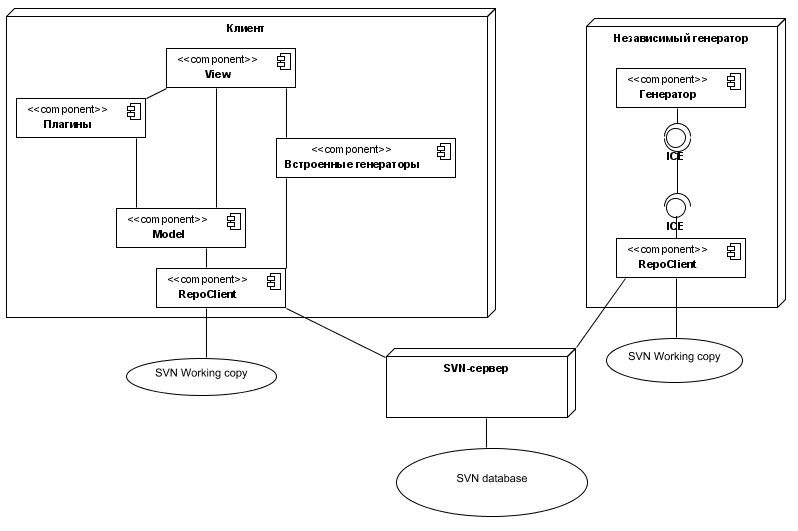
\includegraphics[width=1\textwidth, bb=0 0 798 531]{01-architecture.png}
    \caption{Архитектура CASE-пакета QReal}
    \label{architecture}
  \end{center}
\end{figure}

Для данного исследования потенциальная расширяемость QReal означает в первую очередь то, что и предлагаемое решение по встраиванию в среду 
распознавания и выполнения команд, соответствующих тем или иным жестам, также не должно зависеть от текущего набора графических редакторов. 
К тому же, при разработке нового или уточнении существующего графического языка в метаредаторе QReal новые сущности могут создаваться и 
удаляться довольно активно, поэтому мы должны иметь возможность задания жестов и ассоциирования их с определенными элементами еще на стадии
создания метамодели, причем эти процессы должны проходить при минимальном участии разработчика языка (например, только если он хочет 
отключить какой-либо жест или его подправить). Все необходимые для распознавания данные должны автоматически создаваться при генерации 
исходного кода плагина по соответствующим метамоделям и не должны требовать значительных вычислительных ресурсов.

Помимо этого, предлагаемое решение должно обеспечивать простоту генерируемых жестов. Нарисовать жест мышью должно быть проще и быстрее, 
чем выполнить традиционные для многих CASE-пакетов операции по созданию объекта. 

Большинство элементов в визуальных языках имеют представления на диаграммах, состоящие из довольно небольшого набора базовых графических 
примитивов: эллипсов, прямоугольников, линий и их сочетаний. Для таких несложных элементов было бы логично потребовать, чтобы жест, 
соответствующий их созданию, визуально напоминал графическое представление данного объекта. Это позволило бы пользователю CASE-системы 
сэкономить время и силы на запоминание большого числа жестов и сделало бы процесс их использования более естественным. 

\section{Обзор и выбор алгоритмов распознавания}
Задача компьютерного распознавания образов не нова -- задачи идентификации и классификации предметов решают уже более сорока лет. За это 
время было разработано множество алгоритмов и подходов к решению самых разных задач распознавания, однако независимо от класса 
рассматриваемых задач или предметной области все подходы так или иначе состоят из трех этапов: 
\begin{itemize}
  \item анализ и/или измерение объектов;
  \item выделение их характеристических признаков;
  \item классификация объектов в соответствии с полученными признаками.
\end{itemize}

\subsection{Этап измерения}
Для жестов мышью наиболее близкой областью является распознавание одиночных символов или текста в целом. Основной задачей первого этапа 
(``измерение'') является выделение траектории жеста. Применительно к решаемой задаче построение траектории сводится к отслеживанию 
перемещения координат курсора мыши, что не представляет сложностей в реализации. 

\subsection{Выделение признаков}

Большинство существующих алгоритмов распознавания работают с векторами характеристик объектов, которые позволяют абстрагироваться
от несущественных для решаемой задачи признаков, например, таких, как положение и размер. 
В нашем случае каждому жесту соответствует траектория движения курсора мыши -- список точек. Однако, использовать списки точек в качестве
характеристических векторов не удается, так как при переносе или масштабировании жеста их координаты могут меняться довольно сильно.
Некоторые существующие реализации предлагают следующее решение проблемы: сопоставим каждому жесту ключ-строку и будем сравнивать не 
списки точек траекторий, а ключи, им соответствуюшие.

Наиболее очевидным подходом построения ключа является отслеживание изменений ориентации участков жеста относительно выбранной системы координат. 
Участку жеста соответствует угол на плоскости, который попадает в один из диапазонов, а каждому из диапазонов 
углов ставится в соответствие символ в алфавите (см. рис.~\ref{chaos}). 

\begin{figure} [ht]
  \begin{center}
    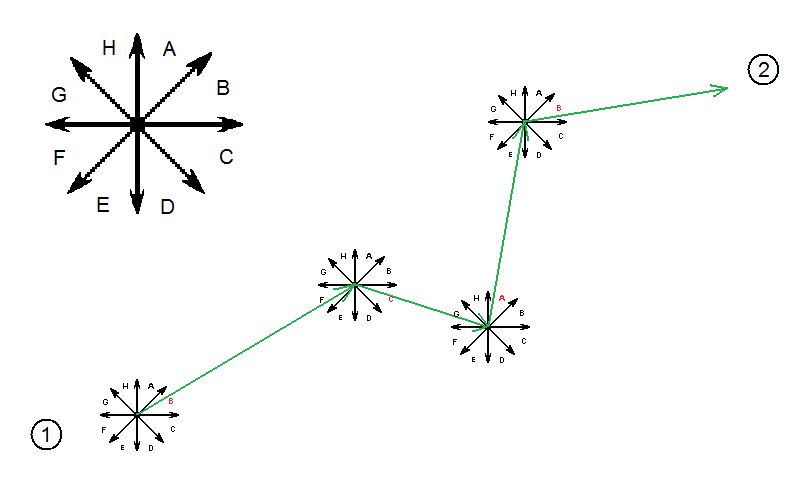
\includegraphics[width=0.7\textwidth, bb=0 0 544 390]{02-chaos.png}
    \caption{Построение ключа по принадлежности направлению}
    \label{chaos}
  \end{center}
\end{figure}

Путь мыши при этом представляется как последовательность символов, соответствующих каждому из направлений. Недостаток этого алгоритма состоит 
в том, что даже небольшое дрожание руки, породившее короткий отрезок в неправильном направлении, добавит в ключ-строку новый символ, что
может привести к ложному распознаванию жеста.

Другой алгоритм предлагает рассматривать не принадлежность направлению, а принадлежность прямоугольнику. Вокруг траектории законченного жеста 
описывается прямоугольник, каждая сторона которого делится на 8 частей (см. рис.~\ref{squares}). Каждому внутреннему 
прямоугольнику ставится в соответствие символ алфавита. Строка-ключ жеста будет состоять из символов, соответствующих прямоугольникам, по
которым проходит трактория жеста. После удаления подряд идущих одинаковых символов из строки получаем окончательный ключ текущего жеста. 

\begin{figure} [ht]
  \begin{center}
    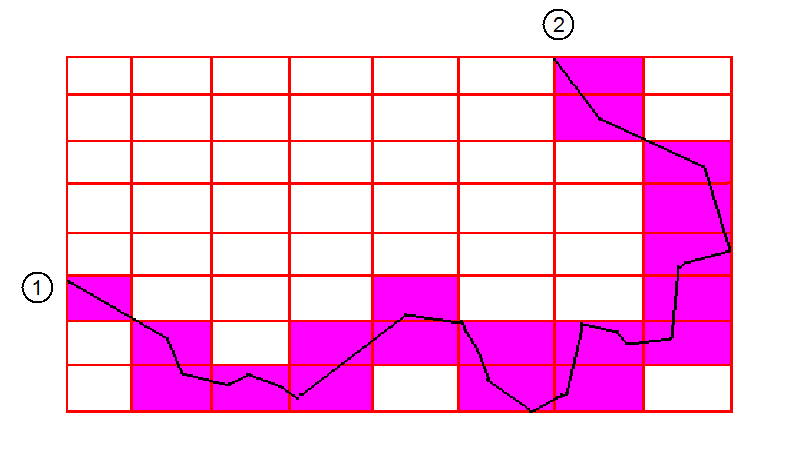
\includegraphics[width=0.8\textwidth, bb=0 0 544 390]{03-squares.png}
    \caption{Построение ключа по принадлежности прямоугольнику}
    \label{squares}
  \end{center}
\end{figure}

Этот алгоритм хорош тем, что при его использовании не надо масштабировать жест. Подобным фигурам будут соответствовать одни и те же ключи.

Подряд идущие повторяющиеся символы можно не удалять, но тогда жест придется приводить к заранее определенному стандартному размеру. 
Но в этом случае при уменьшнении некоторых ломаных может оказаться, что некоторые их части становятся слишком маленькими и
могут быть на этапе фильтрации приняты за шум.


\subsection{Классификаторы}

Для различения жестов используются специальные математические модели, называемые классификаторами. Получая на вход вектор признаков,
классификатор сообщает, к какому классу объектов принадлежит данный объект. 

Среди используемых подходов к классификации наибольшей популярностью в задачах распознавания является 
использование таких математических моделей, как искусственные нейронные сети~\cite{neuronet1, neuronet2, neuronet3}, 
скрытые марковские модели~\cite{hmm1, hmm2, hmm3}, а также классификаторов, получаемых обучением с помощью, например, 
метода опорных векторов~\cite{svm1, svm2} или алгоритмов AdaBoost/FloatBoost~\cite{boosting1, boosting2}.
Принцип работы у всех этих классификаторов примерно одинаковый -- вначале осуществляется фаза обучения, на которой классификатору на вход
подается набор эталонных объектов, соответствующих каждому классу. В рабочем режиме обученный классификатор сопоставляет входные вектора 
признаков классу, соответствующему данным объектам.

Налачие этапа обучения для нашей задачи недопустимо, поскольку в процессе метамоделирования новые сущности могут появляться
довольно часто, а обучение требует наличия большой базы примеров (например, набора типичных траекторий для каждого жеста). Такую
базу невозможно создать в короткие сроки при быстрой разработке предметно-ориентированного языка. 
Данное ограничение является довольно серьезным и, к сожалению, не позволяет нам использовать данный класс классификаторов для решения 
поставленной задачи.

Другим часто используемым в машинном обучении подходом к классификации объектов является так называемая задача поиска ближайшего 
соседа~\cite{nns1, nns2}, заключающийся в отыскании среди множества элементов, расположенных в некоем метрическом пространстве (в 
общем случае, многомерном), элементов, близких к заданному, согласно некоторой функции близости. 
В случае представления траекторий строками из некоторого алфавита в качестве функции близости можно взять расстояние Левенштейна, 
которое определяется как минимальное количество операций вставки одного символа, удаления одного символа и замены 
одного символа на другой для превращения одной строки в другую [88]. Расстояние Левенштейна обладает следующим недостатком:
расстояния между совершенно разными короткими строками оказываются небольшими, а расстояния между похожими длинными словами 
оказываются значительными. Поэтому мы будем сравнивать не само расстояние, а соотношение 

\begin{equation}
\label{levenshtein}
d_{normalized}(s1,s2) = \frac{d(s1,s2)}{min(s1,s2)},
\end{equation}

где d(s1,s2) -- расстояние Левенштейна между строками s1 и s2, а min(s1,s2) -- минимум длин этих строк.

Важным элементом алгоритмов такого рода является понятие набора эталонов -- объектов, с которыми сравнивается входной набор признаков при 
поиске ближайшего соседа. В нашем случае эталонные вектора признаков будут строиться по так называемым ``идеальным жестам'' -- жестам,
генерируемым на основе графического представления элементов. 

Для каждого объекта в QReal есть графическое представление, которое задается с помощью текстового языка на основе XML ~\cite{qrealBasic}. 
Пподобное описание элемента представляет собой набор отрезков, каждый из которых определяется координатами начала и конца, и
набор окружностей, которые определяются координатами диаметра (для того, чтобы работать только с отрезками, окружность при 
равномерном движении мыши можно приближать правильным многоугольником). 

Таким образом, для каждого объекта можно выделить набор вершин (концы всех отрезков и точки на окружности) и ребер (отрезки) и 
построить по ним граф, соответствующий объекту. Построение ``идеальных жестов'' основано на понятии эйлерова пути графа --  
пути, проходящем по всем ребрам графа, причем по каждому из них только по одному разу. 
Если в полученном графе объекта эйлеров путь не существует, добавим несколько ребер так, чтобы эйлеров путь существовал. 
Добавлять будем ребра, связывающие два подграфа, в которых уже существуют эйлеровы пути.

Полученный эйлеров путь и будем считать ``идеальным жестом'' для данного объекта. 


\subsection{Алгоритм распознавания жестов без генерации строки-ключа}

При создании QReal использовуется инструментарий Qt~\cite{qt}, разработчиками которого предложен свой алгоритм распознавания жестов мышью~\cite{qtGestures},
не требующий в процессе работы построения строки-ключа и основанный на анализе изменения направлений участков жеста. Рассмотрим шаги алгоритма:
\begin{enumerate}
  \item Фильтрация пути мыши.
  \item Сопоставление объекта из списка. Предполагается, что объект в этом алгоритме -- это ломаная.
  \begin{enumerate}
    \item Приближение направлениями. На этом этапе каждый сегмент ломаной приближается одним из заранее определенных базовых направлений. 
Как правило, их 4 – вверх, вниз, вправо, влево. Для большей точности количество базовых направлений можно увеличить, при этом удобно 
брать число, кратное 4, чтобы 4 базовых направления оставались неизменными, и каждое было биссектрисой двух соседних. При увеличении числа 
направлений к жестам можно добавлять сложные многоугольники, стороны которых не обязательно параллельны осям координат, которые было бы 
невозможно распознать в случае использования только четырех направлений.
    \item Упрощение списка направлений, заключающееся в том, чтобы найти подряд идущие соноправленные вектора и объединить их в 
один вектор, просуммировав длину.
    \item Сопоставление и удаление. Эта часть алгоритма является, пожалуй, наиболее сложной, так как, несмотря на фильтрацию, останутся 
мелкие сбои вдоль длинных отрезков. На этом шаге списку направлений сопоставляется команда. Если для списка нет команды, мы удаляем 
кратчайший отрезок и повторяем попытку. Алгоритм заканчивается, если удалось получить команду, или большая часть первоначального списка 
направлений была удалена.
  \end{enumerate}
\end{enumerate}

Недостаток этого алгоритма состоит в том, что изменение оставшихся отрезков после удаления самого короткого довольно нетривиально. 
Чтобы путь не потерял связность, удалить отрезок, не изменив концы соседних с ним, невозможно. Чтобы отрезки сохранили свое направление, 
придется менять не только соседние. Например, на рис.~\ref{qt}a показана часть пути мыши. После удаления самого короткого отрезка с номером 2, 
переносим отрезок номер 3, тем самым меняя координаты начала отрезка номер 4. Путь преобразуется в траекторию, приведенную на рис.~\ref{qt}b.
Стоит заметить, что при увеличении числа направлений перестраивать путь будет все сложнее. 

\begin{figure} [ht]
  \begin{center}
    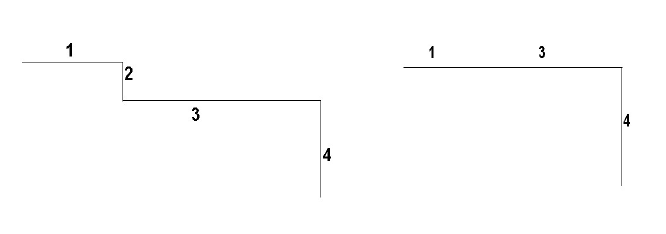
\includegraphics[width=0.8\textwidth, bb=0 0 500 200]{04-qt.png}
    \caption{Объединение участков пути}
    \label{qt}
  \end{center}
\end{figure}

[сравнение]

\subsection{Предлагаемый подход}

Исходя из рассмотренных алгоритмов распознавания, а также в соответствии со спецификой задачи был выбран следующий подход к ее решению:

\begin{itemize}
  \item CASE-система получает сигналы о том, что пользователь зажал правую кнопку мыши и перемещает курсор, и сохраняет координаты положения курсора
через равные промежутки времени. Жест считается завершенным, когда пользователь отпускает кнопку мыши.
  \item Осуществляется сглаживание полученной траектории. Этот шаг необходим, так как различное оборудование дает разную точность при получении 
позиции курсора. Кроме того, если учитывать все дрожания руки, придется усложнять следующий шаг -- сопоставление объекта: каждому объекту
будет соответствовать слишком много разных вариантов пути мыши.
  \item Списку точек сопоставляется строка в соответствии с алгоритмом, отраженным на рис. 3. [может его как-то поименовать?]
  \item С помощью модифицированного алгоритма Левенштейна находится идеальный ключ, расстояние $d_{normalized}$~(\ref{levenshtein}) между которым и 
сгенерированным по нарисованному жесту наименьшее. Если ключ достаточно близок к идеальному, на диаграмме создается объект, соответствующий этому ключу.
\end{itemize}


\section{Реализация}

В реализации QReal список идеальных жестов создается на этапе генерации плагина. Изображенный пользователем жест сравнивается с идеальными, 
после чего генерируется наиболее подходящий элемент в центре изображенного жеста. 

Возникает проблема похожести жестов: идеальный жест генерируется по описаню графического представления объекта. Если графически объекты похожи, 
то и идеальные жесты будут похожи. В пределах одного редактора похожие [начинает бесить слово "похожие", малоразличимые, одинаковые?] идеальные 
жесты можно редактировать вручную: вводится операция вращения и некоторые жесты предлагается рисовать по часовой стрелке, а некоторые --
 против. Решение о вращении идеального жеста в настоящее время принимает разработчик, впоследствии операция вращения может быть автоматизирована. 
Но одной только операцией вращения не обойтись, так как в разных редакторах могут слишком часто встречаться объекты с аналогичным графическим 
представлением. Если жесту пользователя соответствует несколько элементов, то будет вызываться меню со списком возможных элементов, из 
которого пользователь выберет нужный[хотя мы так мечтали избавиться от менюшек...]. На данный момент в QReal в качестве списка идеальный 
жестов загружается список жестов, соответствующих элементам корневой диаграммы. Корневая диаграмма - диаграмма, соответствующая текущему 
табу [кто-то что-то поймет?]. В будущем предполагается создавать список идеальных жестов, соответствующих всем элементам из загруженных 
редакторов.

Кроме объектов с заданным графическим представлением, в QReal входят связи, соединяющие два объекта. В описании редакторов содержится какие 
связи какие объекты могут соединять. Мышиный жест, порождающий связь, - кривая, соединяющая два объекта. По объекту, из которого выходит 
мышиный жест, и объекту, в который жест входит, получаем список возможных связей. А пользователь выбирает необходимую ему связь.

На даннный момент в QReal около 95\% ложно-положительных срабатываний.

\section{Направления дальнейшего исследования}

модификация функции левенштейна для весов

\pagebreak

\begin{thebibliography}{99}
  \bibitem{qrealBasic} А.Н. Терехов, Т.А. Брыксин, Ю.В. Литвинов и др., Архитектура среды визуального моделирования QReal. // Системное 
программирование. Вып. 4: Сб. статей / Под ред. А.Н.Терехова, Д.Ю.Булычева. --- СПб.: 2009, с. 171-196
  \bibitem{strokeIt} StrokeIt, URL: http://www.tcbmi.com/strokeit/  
  \bibitem{gMote} gMote, URL: http://www.handform.net/gmote.php
  \bibitem{xstroke} xstroke, URL: http://freshmeat.net/projects/xstroke/
  \bibitem{flyGesture} FlyGesture, URL: http://flyingmeat.com/flygesture/
  \bibitem{neuronet1} Bishop, C.M., Neural Networks for Pattern Recognition, Oxford: Oxford University Press, 1995
  \bibitem{neuronet2} Ripley, B.D., Pattern Recognition and Neural Networks, Cambridge University Press, 1996
  \bibitem{neuronet3} FaaborgUsing, A.J., Using Neural Networks to Create an Adaptive Character Recognition System, Cornell University, Ithaca, NY, 2002
  \bibitem{hmm1} Rabiner, Lawrence R., A tutorial on hidden Markov models and selected applications in speech recognition, Proceedings of the IEEE, 1989, pp. 257-286
  \bibitem{hmm2} Starner, T., Pentland, A., Visual Recognition of American Sign Language Using Hidden Markov Models, MIT, 1995
  \bibitem{hmm3} Vlontzos, J.A., Kung, S.Y., Hidden Markov models for character recognition, IEEE Transactions on Image Processing, 1992
  \bibitem{svm1} Aizerman, M., Braverman, E., Rozonoer, L., Theoretical foundations of the potential function method in pattern recognition learning., 
Automation and Remote Control 25, 1964, pp. 821–837
  \bibitem{svm2} Catanzaro, B., Sundaram N., Keutzer K., Fast Support Vector Machine Training and Classification on Graphics Processors, International 
Conference on Machine Learning, 2008
  \bibitem{boosting1} Freund, Y., Schapire, R.E., A Short Introduction to Boosting, AT\&T Labs Research, 1999
  \bibitem{boosting2} Li, S.Z., Zhang, Z., FloatBoost Learning and Statistical Face Detection, IEEE Transactions on Pattern Analysis and Machine Intelligence, 2004
  \bibitem{nns1} Potamias, M., Athitsos, V. , Nearest Neighbor Search Methods for Handshape Recognition, PETRA, 2008
  \bibitem{nns2} Shakhnarovish, Darrell, and Indyk, Nearest-Neighbor Methods in Learning and Vision, MIT Press, 2005
  \bibitem{qt} Qt, URL: http://qt.nokia.com/
  \bibitem{qtGestures} Thelin, J., Recognizing mouse gestures, Qt online reference documentation, URL: http://doc.trolltech.com/qq/qq18-mousegestures.html 
\end{thebibliography}
  

\end{document}






